\section{An adaptive algorithm}
\label{sec:adaptive}
We introduce in this section an adaptive algorithm for the case when an optimal sequence of polynomial subspaces, the rate of convergence $\rs_l\to \rs_{\infty}$, or the cost for evaluations of $\rs_l$ are unknown. 

To describe our algorithm, we restrict ourselves to the case when $\domPS=[0,1]^{\dps}$, $\dps\in\N$ and when $\measure=\lambda$ is the Lebesgue measure.
 By the results in \Cref{ssec:arcsine}, we may then use samples and weights from the arcsine distribution instead of the optimal distributions. This allows us to keep previous samples when we extend the polynomial subspaces, whereas using the optimal distribution, which depends on the polynomial subspace, would require throwing away all samples each time the polynomial subspace is extended.
 
 We next describe the building blocks that are used by our adaptive algorithm to select polynomial approximation subspaces.
\begin{definition}[\textbf{Multivariate Legendre polynomials}]\leavevmode
\begin{enumerate}[(i)]
	\item We denote by $(\leg_i)_{i\in\N}$ the univariate $L^2_{\lambda}([0,1])$-orthonormal Legendre polynomials and define their tensor products
	\begin{equation*}
	\begin{split}
	\leg_{\mip}:=\bigotimes_{j=1}^\dps\leg_{\mip_j}\colon [0,1]^d\to\R,\\
	\leg_{\mip}(\psmi):=\prod_{j=1}^{d}\leg_{\mip_j}(\psmi_j)
	\end{split}
	\end{equation*}
	 for $\mip\in\N^\dps$.
\item For each multi-index $\mi\in\N^{d}$, we define the polynomial subspace
\begin{equation*}
\pss_{\mi}:=\vspan\{\leg_{\mip}:2^{\mi}-1\leq\mip< 2^{\mi+1}-1\}\subset L^2([0,1]^d,\lambda).
\end{equation*}

 %For multi-index sets $\mathcal{J}\subset\N^{d}$, we define the orthogonal sums
%\begin{equation*}
%\pss_{\mathcal{J}}:=\bigoplus_{\mi\in\mathcal{J}}\pss_{\mi}\subset L^2_{\lambda}([0,1]^d),
%\end{equation*}
%with the convention $\pss_{\varnothing}=\{0\}$.
\end{enumerate}
\end{definition}
\begin{rem}[\textbf{Orthonormal decomposition}]
	Since polynomials are dense in $L^2_{\lambda}([0,1]^d)$, the subspaces $(\pss_{\mi})_{\mi\in\N^d}$ form an orthonormal decomposition of $L^2_{\lambda}([0,1]^d)$. 	We use exponentially large subspaces instead of the simpler, one-dimensional subspaces $\pss_{\mi}=\R\cdot\leg_{\mi}$ to avoid computational overhead resulting from slow construction of large polynomial subspaces.
\end{rem}
We use the notation $\rs_{-1}:=0$ to avoid separate treatment of the term corresponding to $l=0$ in the following.
To describe a multilevel approximation, %of the form
 we need to construct a sequence $(\vsp_k)_{k=0}^{L}$ of polynomial subspaces, such that the difference $\rs_{l}-\rs_{l-1}$ is projected onto $\vsp_{L-l}$ using weighted least squares approximation. The final approximation is then defined as 
  \begin{equation}
  \label{eq:adaptive}
  \sum_{l=0}^{L}\P_{{L-l}}(\rs_l-\rs_{l-1}).
  \end{equation}
  where $\P_{k}$ projects onto $\vsp_{k}$ for $0\leq k\leq L$.
% Since the total number of levels will not be known beforehand, we denote this subspace by $\vsp_l$, instead of $\vsp_{L-l}$ as before. In particular, the sequence of polynomial subspaces $\vsp_{l}$ used by the adaptive algorithm will be \emph{decreasing}, not increasing, and the final approximation will be of the form
% \begin{equation}
 %\label{eq:adaptive}
 %\sum_{l=0}^{\infty}\P_{l}(\rs_l-\rs_{l-1}), 
 %\end{equation}
 %list of function values $\{(\rs_{l}-\rs_{l-1})(\psmi_{j,l}):\psmi_{j,l}\in\domPS_l\subset\domPS\}$ and a polynomial subspace $\vsp_{l}\subset L^2_{\lambda}([0,1]^d)$ 
 %where $\Pi_{l}$ projects onto $\vsp_{l}$. 
As in \Cref{sec:nonadaptive}, if the samples used by $\P_{{k}}$ are distributed according to the optimal distribution of $\vsp_{k}$, then we require that the number of samples $\NS_{k}$ satisfy
 \begin{equation}
 \label{eq:adaptivestability}
 \kappa \frac{\NS_k}{\log \NS_k}\geq \dim \vsp_{k}
 \end{equation}
 for some $\kappa>0$. However, we then have to throw away all samples each time the space $\vsp_{k}$ is extended, as this changes the optimal distribution. As an alternative, we may use samples from the arcsine distribution, which is independent of the polynomial subspaces $\vsp_{k}$ and thus allows us to reuse samples and corresponding function evaluations. By \Cref{ssec:arcsine}, this increases the number of required samples only by a constant factor (that depends exponentially on the dimension $d$, however).\\

  To construct the sequence of polynomial subspaces in an adaptive fashion, our algorithm constructs a (finite) downward closed multi-index set $\mis\subset\N^{d+1}$. Given such a set, we let 
  \begin{equation*}
\vsp_{k}:=\bigoplus_{\mi\in\N^{d}: (\mi,L-k)\in\mis}\pss_{\mi}\quad 0\leq k\leq L,
\end{equation*}
where
\begin{equation*}
L:=\max\{l\in\N:\exists\mi\in\N^{d} \text{ s.t. }(\mi,l)\in\mis\}<\infty,
\end{equation*} 
which means that we project the difference $\rs_l-\rs_{l-1}$ onto the subspace $\vsp_{L-l}$ that is determined by the slice $\mis_{l}:=\{\mi\in\N^d:(\mi,l)\in \mis\}$ of the multi-index set $\mis$.
To construct $\mis$, starting with $\mathcal{I}=\{\mathbf{0}\}$, our algorithm adds one multi-index at a time according to the following procedure, which resembles algorithms for adaptive sparse grid integration \cite{MR2163199,gerstner2003dimension}.
We call
\begin{equation*}
\mia:=\{(\mi,l)\in \N^{d+1}\setminus \mis:\mis\cup\{\mi,l\}\text{ is downward closed}\}
\end{equation*}
the set of \emph{admissible multi-indices}.
\begin{enumerate}[(i)]
	\item
For each admissible multi-index $(\mathbf{k},l)$, we estimate the norm of the projection of $\rs_l-\rs_{l-1}$ onto $\pss_{\mi}$. This estimate represents the gain that is made by adding $(\mi,l)$ to $\mis$.
 Furthermore, we estimate the work that adding this multi-index would incur.
\item We expand $\mathcal{I}$ by the multi-index that maximizes the ratio between the gain and work estimates.
\end{enumerate}
\begin{figure}[ht]
	\centering
	% This file was created by matplotlib2tikz v0.5.15.
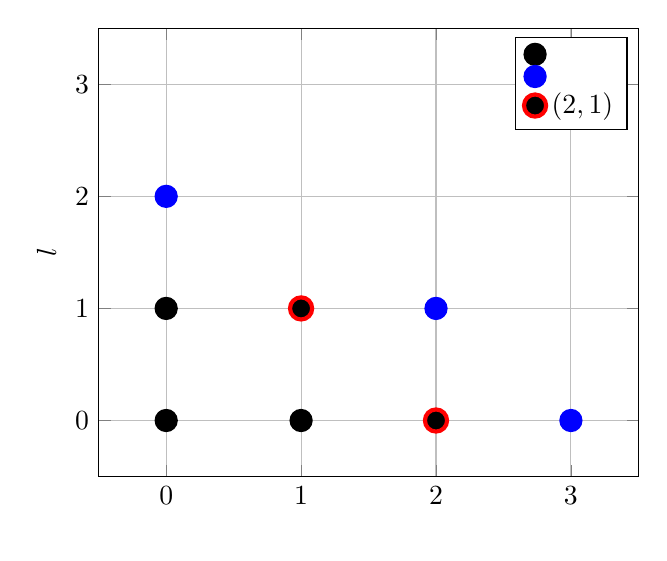
\begin{tikzpicture}

\begin{axis}[
xmin=-0.5, xmax=3.5,
ymin=-0.5, ymax=3.5,
axis on top,
xmajorgrids,
ymajorgrids,
xlabel=$\mi$,
ylabel=$l$
]
\addplot [only marks,mark size=4, draw=black, fill=black]
table {%
x                      y
+0.000000000000000e+00 +0.000000000000000e+00
+1.000000000000000e+00 +0.000000000000000e+00
+0.000000000000000e+00 +1.000000000000000e+00
+2.000000000000000e+00 +0.000000000000000e+00
+1.000000000000000e+00 +1.000000000000000e+00
};
\addplot [only marks, mark size=4,draw=blue, fill=blue]
table {%
x                      y
+3.000000000000000e+00 +0.000000000000000e+00
+2.000000000000000e+00 +1.000000000000000e+00
+0.000000000000000e+00 +2.000000000000000e+00
};
\addplot [only marks,mark size=4,line width=1.5, draw=red, fill=black]
table {%
x                      y
+1.000000000000000e+00 +1.000000000000000e+00
+2.000000000000000e+00 +0.000000000000000e+00
};
\addlegendentry{$\mis$};
\addlegendentry{$\mia$};
\addlegendentry{$\neighbors(2,1)$};
\end{axis}

\end{tikzpicture}
	\caption{Example with $d=1$ of a multi-index set $\mis$ and the associated set of admissible multi-indices $\mia$, as well as neighbors $\neighbors(2,1)$ of  $(2,1)\in\mia$. In this example $L=1$,  $\vsp_{1}=\vspan\{1,\psmi,\dots,\psmi^{6}\}=\vspan\{\leg_0(\psmi),\dots,\leg_{6}(\psmi)\}$, and  $\vsp_{0}=\vspan\{1,\psmi,\psmi^2\}=\vspan\{\leg_0(\psmi),\leg_1(\psmi),\leg_2(\psmi)\}$.}
	\label{fig:dc}
\end{figure}

We next explain how we arrive at the gain and work estimates that are required in step (i).
To estimate the norm of the orthogonal projection of $\rs_l-\rs_{l-1}$ onto $\pss_{\mi}$, we compute the arithmetic average of corresponding estimates for the neighbors $\neighbors(\mi,l)=\{(\mi^{(1)},l^{(1)}),\dots\}$ of $(\mi,l)$ in $\mathcal{I}$. Here, by neighbor we mean elements of $\mis$ that differ from $(\mi,l)$ in a single entry by $1$, see \Cref{fig:dc}.
For each such neighbor, we estimate the norm of the orthogonal projection $\operatorname{Proj}_{\mi^{(j)}}(\rs_{l^{(j)}}-\rs_{l^{(j)}-1})$ of $\rs_{l^{(j)}}-\rs_{l^{(j)}-1}$ onto $\pss_{\mi^{(j)}}$ simply by computing the Euclidean norm of those basis coefficients of $\P_{L-l^{(j)}}(\rs_{l^{(j)}}-\rs_{l^{(j)}-1})$ that belong to $\pss_{\mi^{(j)}}$. (Recall that $\P_{L-l^{(j)}}$ is a discrete projection onto the space $\vsp_{L-l^{(j)}}$ of which $\pss_{\mi^{(j)}}$ is a subspace since $\mi^{(j)}\in\mis_{l^{(j)}}$.)
The final estimate can be expressed as
\begin{equation*}
\frac{1}{|\neighbors(\mi,l)|}\sum_{j=1}^{|\neighbors(\mi,l)|}\norm{\operatorname{Proj}_{\mi^{(j)}}\P_{L-l^{(j)}}(\rs_{l^{(j)}}-\rs_{l^{(j)}-1})}{L^2_{\lambda}([0,1]^d)}.
\end{equation*}


To estimate the work that adding $(\mi,l)$ to $\mis$ incurs, we observe that \Cref{eq:adaptivestability} tells us exactly how many new samples are needed. More specifically, if we denote by $\NS(\mis_{l})$ the minimal solution of \Cref{eq:adaptivestability} for the polynomial subspace determined by $\mis_l$, then the required number of new samples of $\rs_{l}-\rs_{l-1}$ is $\NS(\mis_{l}\cup\{\mi\})-\NS(\mis_{l})$. It therefore remains to determine the  work per sample,  $\work(\rs_{l}-\rs_{l-1})$. If this work is unknown, then we store for each level $l$ an estimate, which we update with the observed computational work divided by the number of generated samples each time $\mathcal{I}_{l}$ changes. The final estimate of the work associated with $(\mi,l)$ is
\begin{equation*}
  \work(\rs_{l}-\rs_{l-1}) \cdot\left(\NS(\mis_{l}\cup\{\mi\})-\NS(\mis_{l})\right).
\end{equation*}

%\Cref{fig:dc} shows an example of $\mis$ and $\mia$ in the case $d=1$. In this case, the polynomial subspaces are simply spaces of polynomials with degree less than or equal to some natural number; more specifically, \Cref{fig:dc} represents the case
\Cref{alg:adaptive} gives a summary of our algorithm in pseudocode.
%\begin{rem}[Alternative multilevel construction]
%From the description of the multilevel method in terms of multi-indices as in \Cref{fig:dc}, one sees that one could alternatively first group all the indices that agree in the $\mi$ component instead of the $l$ component, which would yield approximations of the form
%$$
%\P_{\vsp_{0}}f_{L}+\sum_{l=1}^{L}\P_{\vsp_l\ominus \vsp_{l-1}}\rs_{L-l},
%$$
%where $\vsp_{l}\ominus\vsp_{l-1}$ denotes the orthogonal complement of $\vsp_{l-1}$ %in $\vsp_{l}$.
%\end{rem}


\begin{algorithm}[ht]
\caption{Adaptive multilevel algorithm.}\label{alg:adaptive}
\begin{algorithmic}[1]
		\Function{MLA}{$(\rs_l)_{l\in\N}$,STEPS}
		\State  $\mis\gets \{\mathbf{0}\}$
		\State $X_l\gets \varnothing\;\forall l\in\N$
		\State $\Delta_l\gets 0\;\forall l\in\N$
		\For{$0\leq i<\text{STEPS}$}
			\State $(\mi,l)\gets \argmax_{(\mi,l)\in\mia}\frac{\text{GAIN}((\mi,l),(\Delta_l)_{l\in\N},\mis)}{\text{WORK}((\mi,l),\mis)}$
			\State $N_{+}\gets \NS(\mis_{l}\cup\{\mathbf{k}\})-\NS(\mis_{l})$
			\State $\mis\gets \mathcal{I}\cup\{(\mi,l)\}$
			\For{$0\leq j<N_{+}$}
				\State Generate $\psmi\sim \arcsine_{d}$
				\State $y\gets (\rs_{l}-\rs_{l-1})(\psmi)$
				\State $X_l\gets X_l\cup\{(\psmi,y)\}$
			\EndFor
			\State $\Delta_l\gets \P_{L-l}(\rs_{l}-\rs_{l-1})$
		\EndFor
		\State \Return $\sum_{0\leq l\leq L}\Delta_l$
	\EndFunction
	\item[]
	\Function{GAIN}{$(\mi,l)$,$(\Delta_l)_{l\in\N}$,$\mathcal{I}$}
		\State $s=0$
		\For{$(\mi^{(j)},l^{(j)})\in \neighbors(\mi,l)$}
			\State $s\gets s+\|\operatorname{Proj}_{\mi^{(j)}}\Delta_{l^{(j)}} \|_{L^2_{\lambda}}$
		\EndFor

		\State \Return $s/|\neighbors(\mathbf{k},l)|$
	\EndFunction
	\item[]
	\Function{WORK}{$(\mi,l)$,$\mathcal{I}$}
		\State \Return $\work(\rs_{l}-\rs_{l-1})\cdot\left(\NS(\mis_{l}\cup\{\mi\})-\NS(\mis_{l})\right)$
	\EndFunction

\end{algorithmic}
\end{algorithm}
